\section{ChannelState Struct Reference}
\label{structChannelState}\index{ChannelState@{ChannelState}}
{\tt \#include $<$cmd\_\-issuer.h$>$}

Collaboration diagram for ChannelState:\nopagebreak
\begin{figure}[H]
\begin{center}
\leavevmode
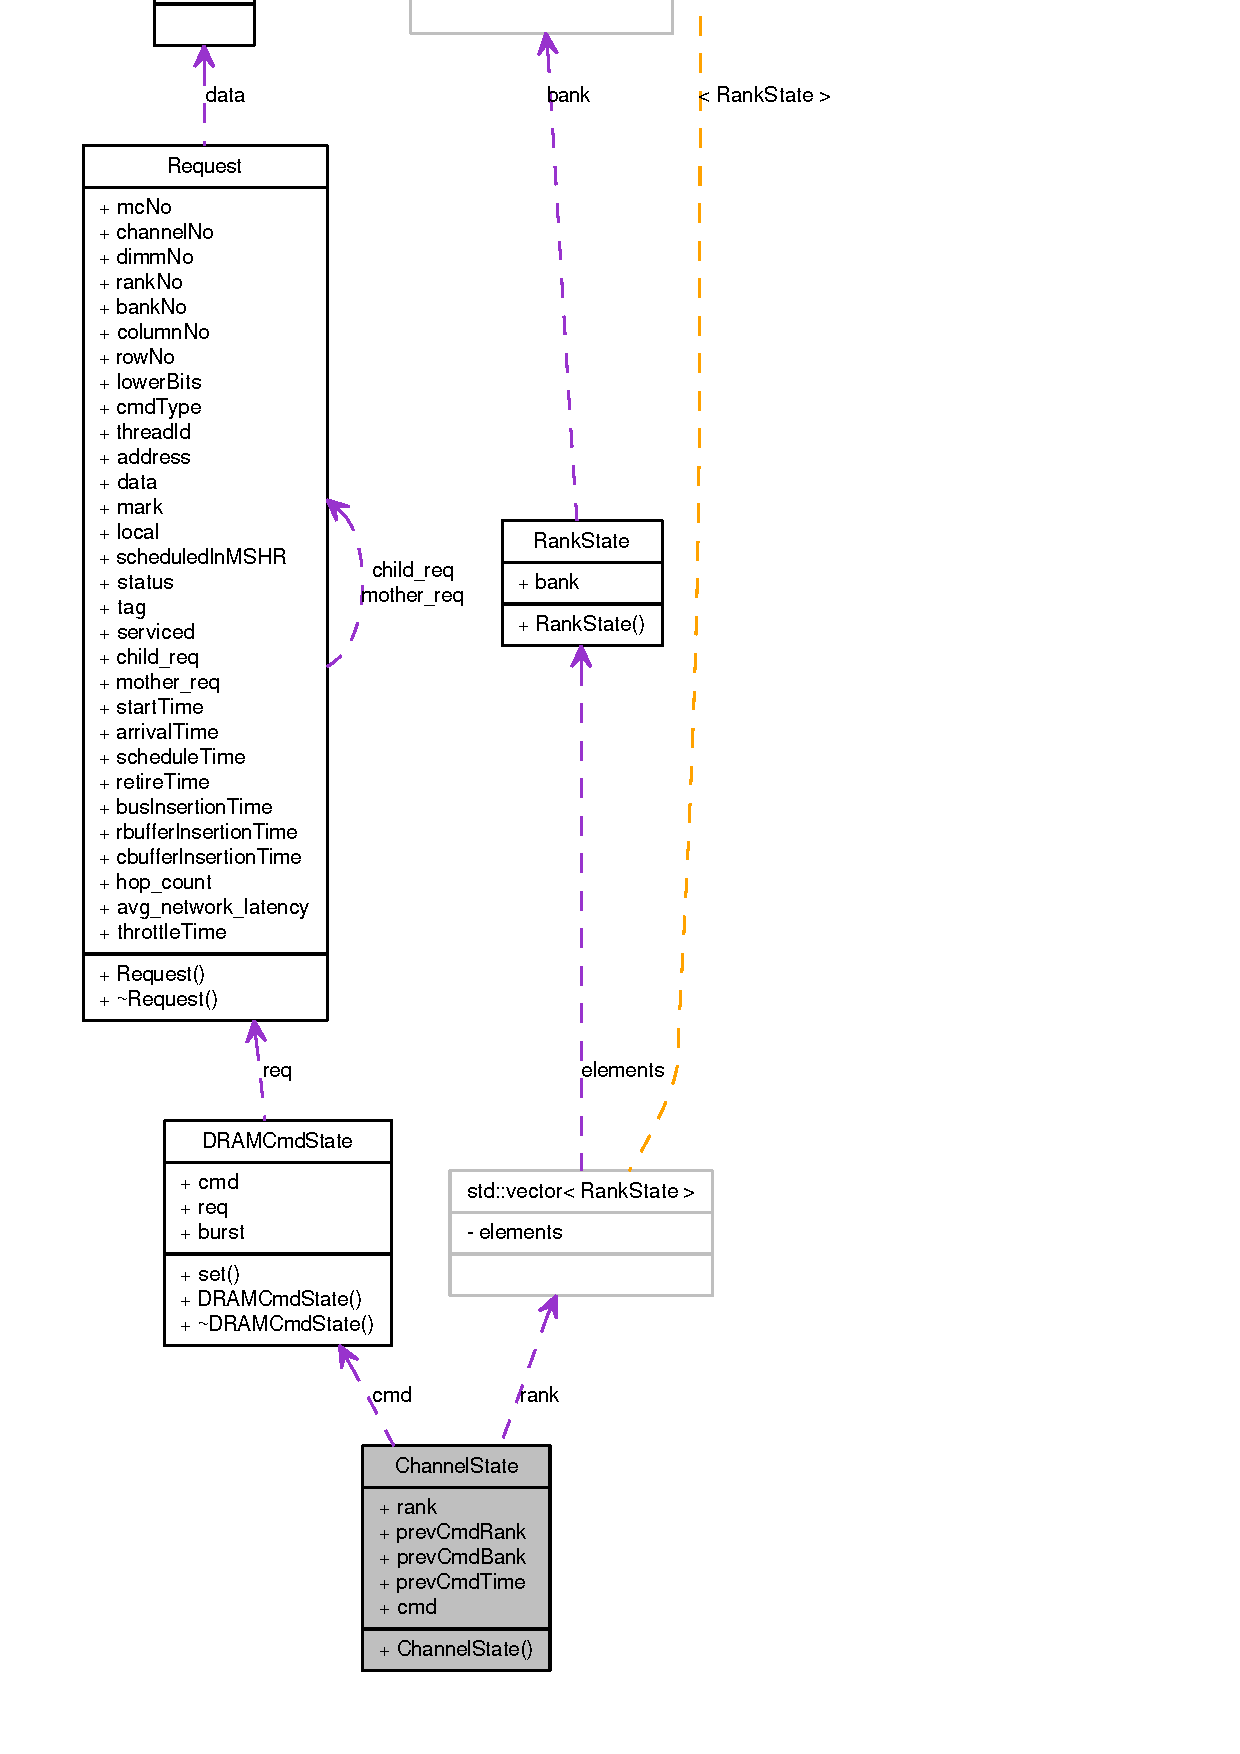
\includegraphics[width=400pt]{structChannelState__coll__graph}
\end{center}
\end{figure}
\subsection*{Public Member Functions}
\begin{CompactItemize}
\item 
{\bf ChannelState} ()
\end{CompactItemize}
\subsection*{Public Attributes}
\begin{CompactItemize}
\item 
vector$<$ {\bf RankState} $>$ {\bf rank}
\item 
unsigned int {\bf prevCmdRank}
\item 
unsigned int {\bf prevCmdBank}
\item 
{\bf Time} {\bf prevCmdTime}
\item 
{\bf DRAMCmdState} {\bf cmd}
\end{CompactItemize}


\subsection{Detailed Description}


Definition at line 100 of file cmd\_\-issuer.h.

\subsection{Constructor \& Destructor Documentation}
\index{ChannelState@{ChannelState}!ChannelState@{ChannelState}}
\index{ChannelState@{ChannelState}!ChannelState@{ChannelState}}
\subsubsection[{ChannelState}]{\setlength{\rightskip}{0pt plus 5cm}ChannelState::ChannelState ()\hspace{0.3cm}{\tt  [inline]}}\label{structChannelState_8f3f06dcef9109fc69d2f62bdc347057}




Definition at line 107 of file cmd\_\-issuer.h.

References NO\_\-OF\_\-RANKS, and rank.

\subsection{Member Data Documentation}
\index{ChannelState@{ChannelState}!cmd@{cmd}}
\index{cmd@{cmd}!ChannelState@{ChannelState}}
\subsubsection[{cmd}]{\setlength{\rightskip}{0pt plus 5cm}{\bf DRAMCmdState} {\bf ChannelState::cmd}}\label{structChannelState_81e9e4a36e784e5438ad12e1e0a517d3}




Definition at line 106 of file cmd\_\-issuer.h.

Referenced by CmdIssuer::BankNotBusy(), CmdIssuer::CmdIssuer(), CmdIssuer::IssueCmd(), and CmdIssuer::SetPrevState().\index{ChannelState@{ChannelState}!prevCmdBank@{prevCmdBank}}
\index{prevCmdBank@{prevCmdBank}!ChannelState@{ChannelState}}
\subsubsection[{prevCmdBank}]{\setlength{\rightskip}{0pt plus 5cm}unsigned int {\bf ChannelState::prevCmdBank}}\label{structChannelState_99e20faf9182a47cb540cb68b72f785f}




Definition at line 104 of file cmd\_\-issuer.h.

Referenced by CmdIssuer::CmdIssuer(), and CmdIssuer::SetPrevState().\index{ChannelState@{ChannelState}!prevCmdRank@{prevCmdRank}}
\index{prevCmdRank@{prevCmdRank}!ChannelState@{ChannelState}}
\subsubsection[{prevCmdRank}]{\setlength{\rightskip}{0pt plus 5cm}unsigned int {\bf ChannelState::prevCmdRank}}\label{structChannelState_4e640c4ef850d6829f93250e61e36307}




Definition at line 103 of file cmd\_\-issuer.h.

Referenced by CmdIssuer::CmdIssuer(), and CmdIssuer::SetPrevState().\index{ChannelState@{ChannelState}!prevCmdTime@{prevCmdTime}}
\index{prevCmdTime@{prevCmdTime}!ChannelState@{ChannelState}}
\subsubsection[{prevCmdTime}]{\setlength{\rightskip}{0pt plus 5cm}{\bf Time} {\bf ChannelState::prevCmdTime}}\label{structChannelState_50665e26c1a30623f91eee4653d3b4c1}




Definition at line 105 of file cmd\_\-issuer.h.

Referenced by CmdIssuer::CanSchedule(), CmdIssuer::CmdIssuer(), and CmdIssuer::SetPrevState().\index{ChannelState@{ChannelState}!rank@{rank}}
\index{rank@{rank}!ChannelState@{ChannelState}}
\subsubsection[{rank}]{\setlength{\rightskip}{0pt plus 5cm}vector$<${\bf RankState}$>$ {\bf ChannelState::rank}}\label{structChannelState_6294b7bb98764df9f1d6fea652602f3e}




Definition at line 102 of file cmd\_\-issuer.h.

Referenced by CmdIssuer::BankNotBusy(), ChannelState(), and CmdIssuer::SetPrevState().

The documentation for this struct was generated from the following file:\begin{CompactItemize}
\item 
{\bf cmd\_\-issuer.h}\end{CompactItemize}
